\documentclass[12pt, titlepage]{article}

\usepackage{booktabs}
\usepackage{tabularx}
\usepackage{hyperref}
\usepackage{graphicx}
\usepackage[normalem]{ulem}
\hypersetup{
    colorlinks,
    citecolor=black,
    filecolor=black,
    linkcolor=blue,
    urlcolor=blue
}
\usepackage[round]{natbib}

\title{SE 3XA3: Software Requirements Specification\\Save The Date}

\author{
        Karuka Khurana (khurak1)\\
        Utsharga Rozario (rozariou)\\
        Samarth Kumar (kumars38)\\
        Dhruv Cheemakurti (cheemakd)\\
        \\
}

\date{\today}

\begin{document}

\maketitle

\pagenumbering{roman}
\tableofcontents
\listoftables
\listoffigures

\newpage

\begin{table}[p]
\caption{\bf Revision History}
\begin{tabularx}{\textwidth}{p{3cm}p{2cm}X}
\toprule {\bf Date} & {\bf Version} & {\bf Notes}\\
\midrule
February 10 & 1.0 & SRS was created\\
February 10 & 1.1 & Non-functional requirements completed\\
February 10 & 1.2 & Project drivers completed\\
February 11 & 1.3 & Project issues completed\\
February 11 & 1.4 & Functional requirements and project constraints completed (SRS Rev.0 complete)\\
March 10 & 1.5 & Functional requirements updated due to outdated source code components\\
\bottomrule
\end{tabularx}
\end{table}

\clearpage

\pagenumbering{arabic}

\newpage

This document describes the requirements for the \textbf{SaveTheDate} project. 
The template for the Software Requirements Specification (SRS) is a subset of the Volere
template ~\citep{RobertsonAndRobertson2012}.

\section{Project Drivers}

\subsection{The Purpose of the Project}
Notion is an all-in-one workspace where users can write, plan, collaborate and organize their thoughts, projects, and other information. Notion has a variety of features that allows users to take notes, add tasks, and even create custom page layouts. Alongside its many features, Notion gives users the ability to upload PDF (Portable Document Format) documents onto a page, providing a built-in view of the document, rather than having to download the PDF every time to view it. Currently, many McMaster students skim through multiple course outlines throughout each semester to jot down or remind themselves of important dates. As a result, students are not only spending extra time reading dense pages of course outlines, but also run the risk of missing important dates and deadlines for different courses.  

With students taking multiple courses per semester, our team would like to automate the process of sifting through documents for due dates and deadlines. We plan to create easy-to-read dashboards for users to quickly access such information for each respective course they are taking. 

\subsection{The Stakeholders}

\subsubsection{The Clients}
The clients of this project are the instructor of SFWRENG 3XA3, Dr. Asghar Bokhari and the teaching assistants (TAs) Stephanie Koehl and Abdul Rab Mohammad. The clients will provide information regarding deadlines for weekly deliverables, insight and guidance when needed and assess how well the application meets requirements.  

\subsubsection{The Customers}
The customers for this product are university students. The customers/users have an influence on the requirements of the application and its overall development since the purpose of the application is intended to help students organize their dates.  

\subsubsection{Other Stakeholders}
The other stakeholders include the team itself, Group 17, and Notion, as we are trying to integrate our application within Notion. Group 17 is an important stakeholder since the entire development and testing process is dependent on the team. 

\section{Project Constraints}
\subsection{Mandated Constraints}
\subsubsection{Solution Design Constraints}

\emph{Description}: The program shall be written in the React.js and Python programming languages.\\
\emph{Rationale}: All developers are familiar with React.js and Python.\\
\emph{Fit Criterion}: The software is written in React.js and Python. \\


\noindent\emph{Description}: The application shall function within Notion. \\
\emph{Rationale}: Notion is a popular organization and management tool used by many students. In addition, the existing project implements Notion with all its features.\\
\emph{Fit Criterion}: All applications are fully operational within Notion.

\subsubsection{Implementation Environment of the Current System}

The application will be cloned from the GitLab repository and executed via the IDE of the user’s choice such as VS Code. To function, the application will be started on the machine.  

\subsubsection{Partner or Collaborative Applications}

\begin{itemize}
  \item[] N/A
\end{itemize}

\subsubsection{Off-the-shelf Software}

\begin{itemize}
  \item[] N/A
\end{itemize}

\subsubsection{Anticipated Workplace Environment}

The product can be used on any desktop machine that can execute React. 

\subsubsection{Schedule Constraints}

\emph{Description}: The project must follow the project schedule shown in the SFWRENG 3XA3 course outline.\\
\emph{Rationale}: The project needs to follow a predefined plan to ensure the completion of deliverables by their respective due dates and the project by the end of the course.\\
\emph{Fit Criterion}: The project will be completed with all the deliverables submitted on time by April 12th, 2022. 

\subsubsection{Budget Constraints}

\begin{itemize}
  \item[] N/A
\end{itemize}

\subsubsection{Enterprise Constraints}

\begin{itemize}
  \item[] N/A
\end{itemize}

\pagebreak

\subsection{Naming Conventions and Technology}

\begin{table}[!hb]
\begin{center}
    \centering
    \begin{tabular}{|l|p{0.72\linewidth}|}
     \hline
     \textbf{Term} & \textbf{Definition} \\
     \hline
     User & The person using the product \\
     \hline
     SRS & Acronym for Software Requirements Specification; A document that describes what the system will do and the expected performance \\
     \hline
     React & A front-end JavaScript library for building user interfaces\\
     \hline
     Tabula-py & Python library for PDF scraping \\
     \hline
     Pandas & Python library for data manipulation \\
     \hline
     Cypress & Front-end testing framework \\
     \hline
     Notion & An organization and project management tool \\
     \hline
     PDF & Portable Document Format \\
     \hline
     PC & A personal computer \\
     \hline
     Scraper & Extracting data from a document or web \\
     \hline
     OS & An operating system\\
     \hline
     Clone & Copy the contents from a repository to local storage  \\
     \hline
     GitLab & A type of Repo for version control \\
     \hline
     Repository & A folder for information \\
     \hline
     Course Outline & A document that informs all students about the assessments, policies, and grading schemes of a specific course \\
     \hline
    \end{tabular}
    \caption{Naming Conventions and Terminology}
    \end{center}
\end{table}

\newpage

\subsection{Relevant Facts and Assumptions}

\subsubsection{Facts}

\begin{itemize}
\item The original repository contains approximately 10,000 lines of code. 
\end{itemize}

\subsubsection{Assumptions}

\begin{itemize}
\item User has already uploaded a PDF using the existing feature to select an upload a PDF to a Notion page. 
\item Users know how to operate a PC.
\item Users understand how to use the features of Notion such as editing a page.
\item Users have access to a PC.
\end{itemize}

\pagebreak

\section{Functional Requirements}

\subsection{The Scope of the Work and the Product}

\subsubsection{The Context of the Work}

  \begin{figure}[!hb]
    \centerline{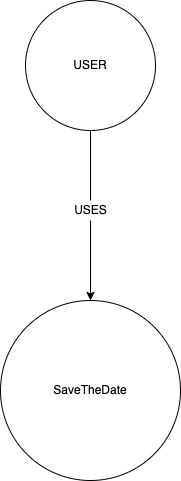
\includegraphics[width=1.5in, height=3in]{images/context_diagram.jpg}}
    \caption{Context Diagram for SaveTheDate}
  \end{figure}

SaveTheDate is a standalone application that does not interact with other systems. It consists of one actor who is the user. 

\pagebreak

\subsubsection{Work Partitioning}

\begin{table}[!ht]
  \begin{center}
    \begin{tabular}{|l|l|l|l|}
      \hline
      Event Number & Event Name         & Input          & Output          \\ \hline
      1            & Select course name & Mouse/Keyboard & N/A             \\ \hline
      2            & Select page range  & Mouse/Keyboard & N/A             \\ \hline
      3            & PDF scraping       & Mouse          & Deadlines       \\ \hline
      4            & Table editing      & Mouse/Keyboard & Changed table   \\ \hline
    \end{tabular}
    \caption{Work Partitioning Events}
  \end{center}
\end{table}


\begin{table}[!htp]
  \begin{center}
    \begin{tabular}{|l|p{0.72\linewidth}|}
      \hline
      Event Number & Summary                             \\ \hline
      1            & The user, through the mouse input and keyboard, can name the course they are choosing to scrape.                                \\ \hline
      2            & The user, through the mouse input and keyboard, can write which pages of the PDF they want scraped.                                 \\ \hline
      3            & The user, through the mouse input, can click a button to scrape the PDF and get the deadlines table in a different Notion page.    \\ \hline
      4            & The user, through the mouse input and keyboard, will be able to edit the deadlines table generated by the PDF scraper.      \\ \hline
      \end{tabular}
      \caption{Work Partitioning Event Summaries}
  \end{center}
\end{table}

\subsubsection{Individual Product Use Cases}

  \begin{figure}
    \centerline{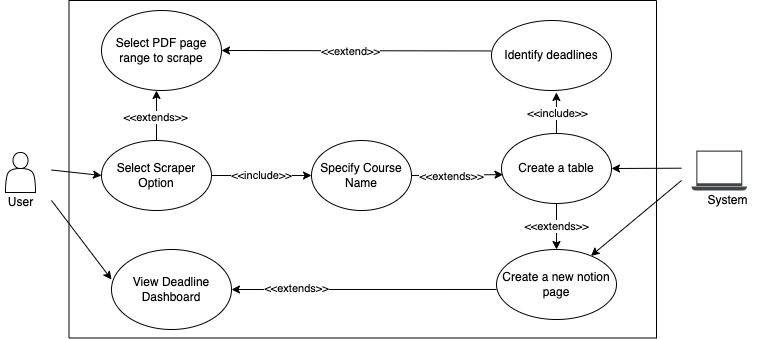
\includegraphics[width=5in, height=2.5in]{images/flow.jpg}}
    \caption{Use case diagram that displays the main functionalities of the application.}
  \end{figure}
  
  The use case diagram shown in Figure 2 illustrates how a can interact with our application. To interact with the application, the user has two main cases. The first one is choosing to scrape a document and the second is to view a pre-existing dashboard of deadlines that have already been scraped from a document. To scrape a document, the user has the ability to provide the system with the page range for the document they want to scrape and to specify the course name. The system will then create a table on a new notion page, identify a table within the document and therefore determine the deadlines. This table will be displayed on the dashboard that the user can access. 

\subsection{Functional Requirements}

\subsubsection{FR1}

\begin{description}
  \item[Description:] The system shall provide the user with a button to begin scraping. 
  \item[Rationale:] The design must be intuitive to use, hence a visual interface for the user. 
  \item[Priority:] High
\end{description}

\subsubsection{FR2}

\begin{description}
  \item[Description:] The system shall have a way to select the page range they want to scrape. 
  \item[Rationale:] If the user knows the range in which the deadlines might exist in the document, the application can scrape over a specified page range, minimizing processing time. 
  \item[Priority:] High
\end{description}

\subsubsection{FR3}

\begin{description}
  \item[Description:] The system shall have a way to identify deadline tables in the PDF.
  \item[Rationale:] It is crucial that the application properly identifies tables with deadlines in a PDF as a PDF might contain a lot of tables irrelevant to deadlines, i.e., tables containing names of professors and their office hours. 
  \item[Priority:] High
\end{description}

\subsubsection{FR4}

\begin{description}
  \item[Description:] The system shall have a way to structure the output table data. 
  \item[Rationale:] The data obtained from a PDF may not be in a table format when read. Hence, there needs to be a way to structure the data into a table before being output in a Notion page. 
  \item[Priority:] High
\end{description}

\subsubsection{FR5}

\begin{description}
  \item[Description:] The system shall have a way to create a Notion table in a page. 
  \item[Rationale:] The application must be able to automatically read the data from the PDF and make a page with the read table. Hence, the system must be able to create a Notion table once it has been given the data for the table. 
  \item[Priority:] High
\end{description}

\subsubsection{FR6}

\begin{description}
  \item[Description:] The system shall display the deadlines as a table in a Notion page. 
  \item[Rationale:] The application should be capable of reading the data and putting it into a Notion table. The table that should be displayed needs to be structured well, in the same if not a better format than that in the PDF. 
  \item[Priority:] High
\end{description}

\subsubsection{FR7}

\begin{description}
  \item[Description:] The system shall make the table editable. 
  \item[Rationale:] The user might think of changing the deadline in a table, for example, if the due date has been changed by the course instructor. Hence, it is crucial that the table created by the application is editable. 
  \item[Priority:] High
\end{description}

\subsubsection{FR8}

\begin{description}
  \item[Description:] The system shall ask the user to input the course name/code for the table. 
  \item[Rationale:] Since the name of the course might not be explicitly listed in a PDF, i.e. a PDF with only deadlines or a shared course having several course codes. We required the user to input the course code to include a tag and title with the table. 
  \item[Priority:] High
\end{description}

\subsubsection{FR9}
\begin{description}
  \item[\sout{Description:}]\sout{ The system shall create a new page when the scraper is used for the first time.  }
  \item[\sout{Rationale:}] \sout{The idea is to have all the deadlines listed in an easy to access page. Hence a central page for all course deadlines. }
  \item[\sout{Priority:}]\sout{ High}
\end{description}

\begin{description}
  \item[Description:] The system shall have a way to upload PDFs
  \item[Rationale:] The application should be capable of uploading PDFs for viewing. The PDF should be displayed as a application component on the page.
  \item[Priority:] High
\end{description}

\subsubsection{FR10}

\begin{description}
  \item[\sout{Description:}] \sout{The system shall allow the user to scrape multiple PDFs into one page.}
  \item[\sout{Rationale:}] \sout{To increase functionality of our application, the user must be able to insert multiple deadlines from different PDFs into the same page. }
  \item[\sout{Priority:}] \sout{High}
\end{description}

\begin{description}
  \item[Description:] The system shall have a way to select PDFs from the local computer to scrape.  
  \item[Rationale:] The application should be capable of selecting PDFs from local storage for scraping. The PDF pages would be scrapped for deadlines. Hence, it is essential.
  \item[Priority:] High
\end{description}

\subsubsection{FR11}

\begin{description}
  \item[Description:] The system shall have a way to upload images
  \item[Rationale:] The application should be capable of uploading images for viewing. The image should be displayed as a application component on the page.
  \item[Priority:] Low
\end{description}

\subsubsection{FR11}

\begin{description}
  \item[Description:] The system shall have a button that has all the available functionalities.
  \item[Rationale:] All the functionalities should be available through the button function.
  \item[Priority:] High
\end{description}


\section{Non-functional Requirements}

\subsection{Look and Feel Requirements}

\subsubsection{Appearance Requirements}

\begin{itemize}
  \item[LF1.] The application shall be consistent with the Notion theme. 
\end{itemize}

\subsubsection{Style Requirements}

\begin{itemize}
  \item[LF2.] The application shall be consistent with the Notion theme. 
\end{itemize}

\subsection{Usability and Humanity Requirements}

\subsubsection{Ease of Use Requirements}

\begin{itemize}
  \item[UH1.] The application must be accessible to the users in an easy-to-access menu.
\end{itemize}

\subsubsection{ Learning Requirements}

\begin{itemize}
  \item[UH2.] The users should be able to use the application without prior experience or training.
\end{itemize}

\subsubsection{Accessibility Requirements}

\begin{itemize}
  \item[UH3.] The application must adhere to the same accessibility range as the Notion application. 
\end{itemize}

\subsection{Performance Requirements}

\subsubsection{Speed and Latency Requirements}

\begin{itemize}
  \item[PE1.] The application shall be able to scrape a PDF within a reasonable time. 
  \item[PE2.] The application shall be able to make a Notion page within a reasonable time. 
\end{itemize}

\subsubsection{ Safety-Critical Requirements}

\begin{itemize}
  \item[] N/A
\end{itemize}

\subsubsection{ Precision or Accuracy Requirements}

\begin{itemize}
  \item[PE3.] The application shall be able to identify tables with deadlines with an 85\% accuracy.
  \item[PE4.] The application shall be able to recreate tables with 90\% accuracy.
\end{itemize}

\subsubsection{ Reliability and Availability Requirements }

\begin{itemize}
  \item[] N/A
\end{itemize}

\subsubsection{ Robustness or Fault-Tolerance Requirements}

\begin{itemize}
  \item[] N/A
\end{itemize}

\subsubsection{ Capacity Requirements}

\begin{itemize}
  \item[] N/A
\end{itemize}

\subsubsection{ Scalability or Extensibility Requirements}

\begin{itemize}
  \item[] N/A
\end{itemize}

\subsubsection{ Longevity Requirements}

\begin{itemize}
  \item[PE5.] The application must be functional with existing software and hardware by May 2022. 
\end{itemize}

\subsection{Operational and Environmental Requirements}

\subsubsection{ Expected Physical Environment}

\begin{itemize}
  \item[OE1.] The system must not require an Internet connection to function correctly.
\end{itemize}

\subsection{Release Requirements}

\begin{itemize}
  \item[RR1.] The product will have a final release on April 10th, 2022. 
\end{itemize}

\subsection{Maintainability and Support Requirements}

\subsubsection{Maintenance Requirements}

\begin{itemize}
  \item[MA1.] The source code must be fully documented, via commenting and class diagrams. 
  \item[MA2.] The source code must all adhere to the same standard style. 
\end{itemize}

\subsubsection{Supportability Requirements}

\begin{itemize}
  \item[MA3.] The project’s main repository shall be made public, to allow users to raise issues. 
\end{itemize}

\subsubsection{Adaptability Requirements}

\begin{itemize}
  \item[MA4.] The application shall be supported by any machine running Windows 7 or newer, macOS Sierra 10.12 or newer, or Linux Ubuntu 16.04 or newer.
  \item[MA5.] The application shall be supported by Chrome 98.0.X, FireFox 97.0 and Microsoft Edge 97.0.X. 
\end{itemize}

\subsection{Security Requirements}

\begin{itemize}
  \item[] N/A
\end{itemize}

\subsection{Cultural Requirements}

\subsubsection{Cultural Requirements}

\begin{itemize}
  \item[CR1.] The system shall not allow users to input course names that are culturally offensive/inappropriate. 
  \item[CR2.] The system shall not allow users to input course names that are in languages asides from English. 
\end{itemize}

\subsection{Legal Requirements}

\begin{itemize}
  \item[] N/A
\end{itemize}

\subsection{Health and Safety Requirements}

\begin{itemize}
  \item[] N/A
\end{itemize}

\section{Project Issues}

\subsection{Open Issues}
There are no major open issues with the \textbf{react-notion-x} repository. A minor issue is the React-Notion collection view calendar is currently unsupported. The last commit was on Jan. 28, 2022.

\subsection{Off-the-Shelf Solutions}
\textbf{SaveTheDate} is the only open-source PDF deadline scraper that is integrated with Notion webpages. There are other PDF scraping tools like \textbf{DocParser} and 
\textbf{Amazon Textract}, however, these are marketed towards businesses that want to scrape PDF data in bulk, and not just deadlines. Furthermore, they are costly to use, and do not produce tables onto a page like Notion.

\subsection{New Problems}
N/A

\subsection{Tasks}
Tasks are assigned and scheduled based on the \href{https://gitlab.cas.mcmaster.ca/se3xa3_l03_g17/se3xa3_l03_g17/-/blob/main/ProjectSchedule/3XA3_L03_G17_GanttChart.pdf}{Gantt chart}.
%\href{run:../ProjectSchedule/3XA3_L03_G17_GanttChart.pdf}{Gantt chart}

\subsection{Migration to the New Product}
N/A

\subsection{Risks}
The main risk will be getting familiar with potentially unknown tools and libraries such as \textbf{tabula-py} and \textbf{pandas} in Python to build the PDF scraper. This will require reading the documentation and referencing existing code which uses these libraries as a starting point. Another risk will be testing, which may be difficult due to a limited amount of test samples for  the PDF scraper. Using front-end testing, such as \textbf{Cypress}, may additionally be unfamiliar to group members.

\subsection{Costs}
This project is based on open-source code and uses free software tools such as Python libraries, and React, so there is no monetary cost. There is an estimated time cost of about 50 hours for development, testing, and documentation.

\subsection{User Documentation and Training}

\subsubsection{Documentation}
\textbf{SaveTheDate}’s repository will contain a README file with a brief description, usage, and installation instructions. There will also be screenshots for user interfacing options. A developer can also see the documented code in the form of an MIS.

\subsubsection{Training}
By following along an example shown in the README file, the user should understand how to use \textbf{SaveTheDate}. Users will be given a reference to learn the basics of Notion if they are unfamiliar. No specific training is required.

\subsection{Waiting Room}
Other additions, should there be additional development time:
\begin{itemize}
  \item Extract deadlines which are not in tables (unstructured)
  \item YouTube integration, where the user can paste a link and has the option to create a Notion video player for that video.
  \item Website preview, where hovering over a link shows a small graphics window of that website’s home page
  \item Generating multiple tables in different Notion webpages
  \item Generating tables of different formats (user can select the output style they want for their deadlines)
\end{itemize}

\subsection{Ideas for Solutions}
N/A

\bibliographystyle{plainnat}

\bibliography{SRS}

\newpage

\section{Appendix}

This section has been added to the Volere template.  This is where you can place
additional information.

\subsection{Symbolic Parameters}

The definition of the requirements will likely call for SYMBOLIC\_CONSTANTS.
Their values are defined in this section for easy maintenance.


\end{document}
